\documentclass[]{article}

% PACKAGES
\usepackage[a4paper, total={6.5in, 9in}]{geometry}
%\usepackage[margin=1in]{geometry}
\usepackage{fancyhdr}
\usepackage[]{biblatex}
\addbibresource{./references.bib}
\usepackage{wrapfig}
\usepackage{graphicx}
\usepackage{float}
\usepackage{hyperref}
\usepackage{transparent}
\usepackage{listings}
\usepackage{color}
\usepackage{amsmath}
\usepackage{color,soul}
\hypersetup{
	colorlinks,
	citecolor=black,
	filecolor=black,
	linkcolor=black,
	urlcolor=black
}
%---------------------------------------------------------
\lstdefinestyle{code}{
	frame=single,
    basicstyle=\ttfamily,
%   \color{red},
	showstringspaces=false,
	stringstyle=\color{green!33!black},
	keywordstyle=\color{blue},
	keywordstyle=[2]\sf\bf,
	keywordstyle=[3]\sf\bf,
	keywordstyle=[4]\sf\bf,
	identifierstyle=\color{black},
	rulecolor=\color{black},
	commentstyle=\it\tt\color{gray}
}


\definecolor{codegreen}{rgb}{0,0.6,0}
\definecolor{codegray}{rgb}{0.5,0.5,0.5}
\definecolor{codepurple}{rgb}{0.58,0,0.82}
\definecolor{backcolour}{rgb}{0.99,0.99,0.99}

\lstdefinestyle{mystyle}{
	backgroundcolor=\color{backcolour},  
	commentstyle=\color{codegreen},
	keywordstyle=\color{blue},
	numberstyle=\tiny\color{codegray},
	stringstyle=\color{codepurple},
	basicstyle=\footnotesize,
	breakatwhitespace=false,        
	breaklines=true,                
	captionpos=b,                    
	keepspaces=true,                
	numbers=left,                    
	numbersep=5pt,                  
	showspaces=false,                
	showstringspaces=false,
	showtabs=false,                  
	tabsize=2
}

\lstset{style=mystyle}
%
%\lstdefinestyle{java}{
%	style=code,
%	language=Java,
%	morekeywords={assert}
%}
%
%\lstset{style=code}
%
%\lstset{language=java}

% HEADER AND FOOTER 
\usepackage{fancyhdr}
\pagestyle{fancy}
\fancyhf{}
\lhead{Jordan Yeo - 17727626}
\rhead{Assignment}
%\chead{Team 8}
\cfoot{\thepage}

%---------------------------------------------------------
% HOUSE KEEPING
\graphicspath{ {./images/} }
\setlength\parindent{0pt}
%---------------------------------------------------------

\begin{document}

% TITLE PAGE
%-------------------------------------------------------------------------------

\begin{titlepage}
	\begin{center}
		\vspace*{1cm}
		\LARGE\textbf{Operating Systems - Assignment}
		\break
		COMP2006
		\vspace{1cm}
		\break
		\Large\textbf{Jordan Yeo \\17727626} 
		\vspace{3cm}

%		\begin{figure}[H]
%		\begin{center}
%			{
%				\includegraphics[height=0.2\textheight,width=1.0
%				\textwidth]{goodbye.png}}
%		\end{center}
%		\end{figure}
		
		\vspace{14.0cm}
		\normalsize
		Curtin University \\
		Science and Engineering \\
%		Perth, Australia \\
%		October 2016
		
	\end{center}
\end{titlepage}

%-------------------------------------------------------------------------------
\tableofcontents
\pagebreak


\pagenumbering{arabic} 
\addcontentsline{toc}{section}{Introduction}
\section*{Introduction}
The following report is for the Operating Systems Assignment for 2017. It will detail how mutual exclusion was achieved for processes and threads. Also the processes and threads that accessed shared resources.
%--------------------------------------------------------
% PART A
\section{Process MSSV}
For this implementation of the solution, mutual exclusion is achieved by having the parent (consumer) wait for all child (producer) processes to complete execution before continuing. This waiting is implemented by having the parent wait for the semParent semaphore before accessing the shared variable, representing the number of child processes finished. Once the parent has finished creating children it will only be reading the value of the shared variable. The semParent semaphore is to prevent the critical section problem. So the child does not write to the variable as the parent reads. Once a child completes execution it waits for the semParent semaphore before acquiring a mutex lock to update a shared resource, indicating it is finished. The parent is forced to wait until the value of the shared variable shows that all children are finished. 
$$
wait(semParent)
$$
$$
\ \ \ \ \ \ \ \ \ \ //\ critical\ section\\ 
$$
$$
signal(semParent)\\ \\
$$
\vspace{0.1cm}

To ensure mutual exclusion for the shared resources (buffer1, buffer2 and counter) the child waited to acquire a mutex lock before entering its critical section to modify the shared resources. Since buffer1 was never modified and only read from this did not require a mutex lock to be obtained before reading. \\
$$
wait(semMutex)
$$
$$
\ \ \ \ \ \ \ \ \ \ //\ critical\ section\\ 
$$
$$
signal(semMutex)\\ \\
$$
\vspace{0.1cm}

The semaphores required (semMutex and semParent), buffer1, buffer2 and counter were implemented using shared memory. The following POSIX shared memory functions were used to create shared memory, and the corresponding functions to close the shared memory: \\
$$
shm\_link()
$$
$$
ftruncate()\\
$$
$$
mmap()\\ 
$$
$$
shm\_unlink() \\
$$
$$
close()\\
$$
$$
munmap()\\ 
$$
	
\vspace{0.2cm}
	
Zombie processes were killed with the use of signal(SIGCHILD, SIG\_IGN).


%\pagebreak
%--------------------------------------------------------
% PART B
\section{Thread MSSV}
To achieve mutual exclusion in the multi-threaded program, the parent (consumer) must wait for all threads (producer) to complete execution. The parent uses \textit{pthread\_lock\_mutex()} to lock the mutex then performs a \textit{pthread\_cond\_wait()} on a condition variable. The condition variable represents how many threads are still executing. \\

Once a thread completes execution, it acquires a mutex lock to alter the condition variable signaling it has finished its task. The thread also performs a conditional wait in the case where the parent is using the shared variable. \\
$$
pthread\_mutex\_lock(\&mutex )
$$
$$
pthread\_cond\_wait(\&use, \&mutex)
$$
$$
pthread\_cond\_signal(\&use);
$$
$$
pthread\_mutex\_unlock(\&mutex)
$$
\vspace{0.2cm}

%\textit{pthread\_mutex\_t} and \textit{pthread\_cond\_t} were used.
In thread MSSV the shared resources are declared as global variables. Threads have access to the variables declared global in the parent. Before a thread could access the shared resources it would first need to acquire a mutex lock. The function \textit{pthread\_lock\_mutex()} blocks the caller if the mutex is in use by another. It can then alter the shared resources, counter and buffer2, before releasing the mutex lock.\\

To allocate the memory for buffer1, buffer2, counter and regions \textit{malloc()} was used. The appropriate \textit{free()} calls were used to free the allocated memory. This was done to ensure memory leaks were not present in the operation of the program. 

\pagebreak
%--------------------------------------------------------
% TESTING
\section{Testing}
\subsection{Method}
To test each implementation of MSSV worked as intended multiple input files were used. With these input files, multiple delays were chosen as well. Input files of various 9x9 numbers were used. Input files were used that were valid, contained one error, contained multiple errors. Also tested were smaller grids than 9x9 and empty files. \\

Testing was performed on the lab machines in various rooms of Building 314, Level 2. 

\subsection{Errors}
There are no known errors in the process MSSV and the thread MSSV. Care has been taken to ensure potential memory leaks are prevented, by using the appropriate measures to free allocated memory. Memory leaks are not present in the testing of each MSSV currently performed.

\subsection{Input Files}

$$
specTest\ =\  
\begin{matrix}
6 & 2 & 4 & 5 & 3 & 9 & 1 & 8 & 7 \\
5 & 1 & 9 & 7 & 2 & 8 & 6 & 3 & 4 \\
8 & 3 & 7 & 6 & 1 & 4 & 2 & 9 & 5 \\
1 & 4 & 3 & 8 & 6 & 5 & 7 & 2 & 9 \\
9 & 5 & 8 & 2 & 4 & 7 & 3 & 6 & 1 \\ 
7 & 6 & 2 & 3 & 9 & 1 & 4 & 5 & 8 \\
3 & 7 & 1 & 9 & 5 & 6 & 8 & 4 & 2 \\
4 & 9 & 6 & 1 & 8 & 2 & 5 & 7 & 3 \\
2 & 8 & 5 & 4 & 7 & 3 & 9 & 1 & 6

\end{matrix}
$$
\vspace{1cm}
$$
testFail\ =\  
\begin{matrix}
\fbox{2} & 2 & 4 & 5 & 3 & 9 & 1 & 8 & 7 \\
5 & 1 & 9 & 7 & 2 & 8 & 6 & 3 & 4 \\
8 & 3 & 7 & 6 & 1 & 4 & 2 & 9 & 5 \\
1 & 4 & 3 & 8 & 6 & 5 & 7 & 2 & 9 \\
9 & 5 & 8 & 2 & 4 & 7 & 3 & 6 & 1 \\ 
7 & 6 & 2 & 3 & 9 & 1 & 4 & 5 & 8 \\
3 & 7 & 1 & 9 & 5 & 6 & 8 & 4 & 2 \\
4 & 9 & 6 & 1 & 8 & 2 & 5 & 7 & 3 \\
2 & 8 & 5 & 4 & 7 & 3 & 9 & 1 & 6

\end{matrix}
$$
\vspace{1cm}
$$
multiFail\ =\  
\begin{matrix}
\fbox{2} & 2 & 4 & 5 & 3 & 9 & 1 & 8 & 7 \\
5 & 1 & 9 & 7 & 2 & 8 & 6 & 3 & 4 \\
8 & 3 & 7 & 6 & 1 & 4 & 2 & 9 & 5 \\
1 & 4 & 3 & 8 & 6 & 5 & 7 & 2 & 9 \\
9 & 5 & 8 & 2 & 4 & 7 & 3 & 6 & \fbox{3} \\ 
7 & 6 & 2 & 3 & 9 & 1 & 4 & 5 & 8 \\
3 & 7 & 1 & 9 & 5 & 6 & 8 & 4 & 2 \\
4 & 9 & 6 & 1 & 8 & 2 & 5 & 7 & 3 \\
2 & 8 & 5 & 4 & 7 & 3 & 9 & 1 & 6

\end{matrix}
$$

\break
\subsection{Expected Results}
\textit{specTest}

\begin{lstlisting}[style=code]
row 1 is valid
row 2 is valid
row 3 is valid
row 4 is valid
row 5 is valid
row 6 is valid
row 7 is valid
row 8 is valid
row 9 is valid
9 out of 9 columns are valid
9 out of 9 sub-grids are valid

There are 27 valid sub-grids, and thus the solution is valid
\end{lstlisting}
\vspace{1cm}
\textit{testFail}
\begin{lstlisting}[style=code]
row 1 is invalid
row 2 is valid
row 3 is valid
row 4 is valid
row 5 is valid
row 6 is valid
row 7 is valid
row 8 is valid
row 9 is valid
8 out of 9 columns are valid
8 out of 9 sub-grids are valid

There are 24 valid sub-grids, and thus the solution is invalid
\end{lstlisting}

\vspace{1cm}
\textit{multiFail}
\begin{lstlisting}[style=code]
row 1 is invalid
row 2 is valid
row 3 is valid
row 4 is valid
row 5 is invalid
row 6 is valid
row 7 is valid
row 8 is valid
row 9 is valid
7 out of 9 columns are valid
7 out of 9 sub-grids are valid

There are 21 valid sub-grids, and thus the solution is invalid
\end{lstlisting}
\subsection{Actual Results}


	\begin{figure}[H]
	\caption{Processes: specTest}
	\begin{center}
		{
			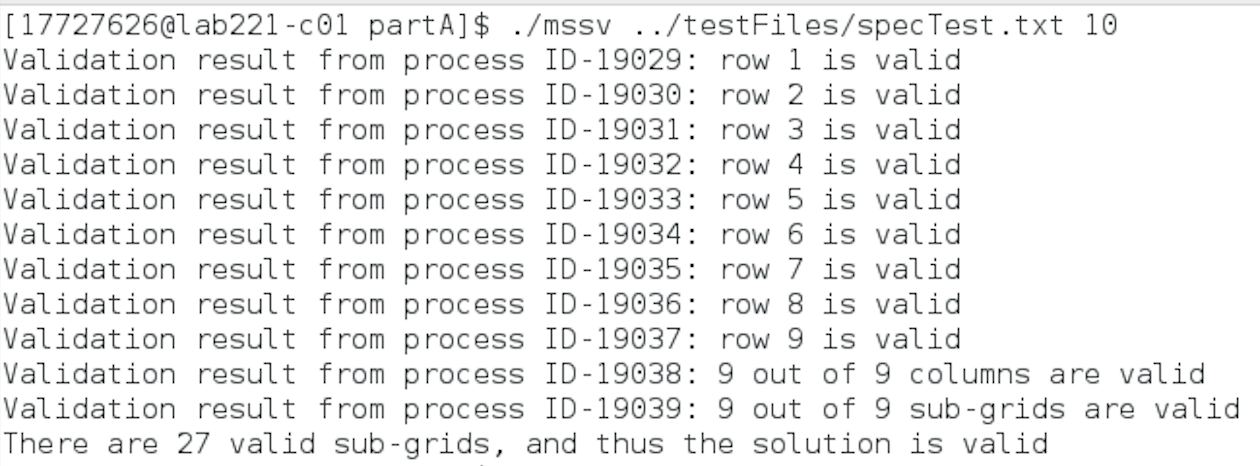
\includegraphics[height=0.25\textheight,width=1.0
			\textwidth]{Pro_spec.png}}
	\end{center}
	\end{figure}
	
	
	\begin{figure}[H]
	\caption{Threads: specTest}		
		\begin{center}
			{
				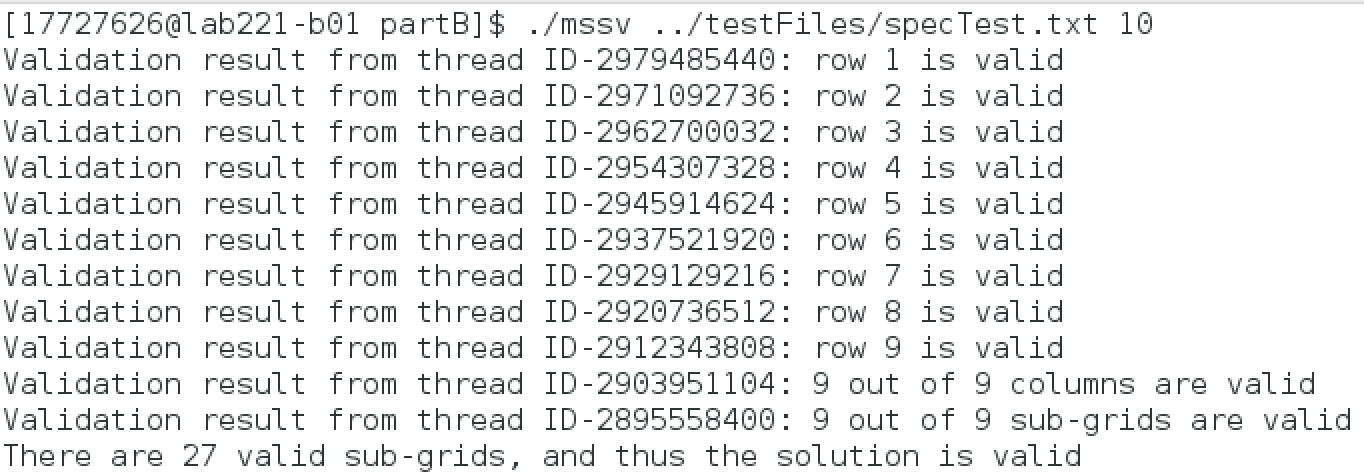
\includegraphics[height=0.25\textheight,width=1.0
				\textwidth]{Thr_spec.png}}
		\end{center}
	\end{figure}

	\begin{figure}[H]
	\caption{Processes: testFail}
	\begin{center}
		{
			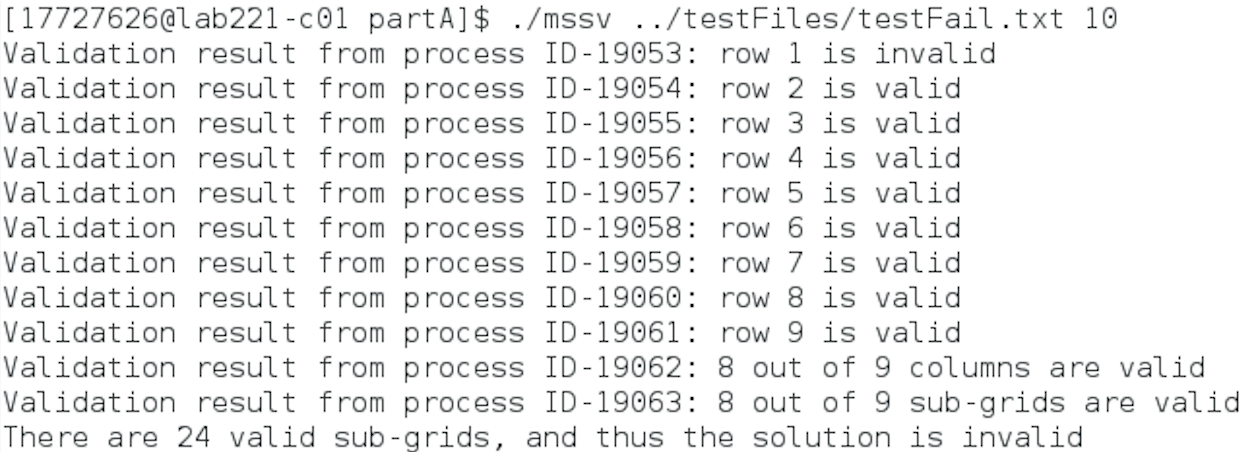
\includegraphics[height=0.25\textheight,width=1.0
			\textwidth]{Pro_testF.png}}
	\end{center}
	\end{figure}


	\begin{figure}[H]
	\caption{Threads: testFail}		
	\begin{center}
		{
			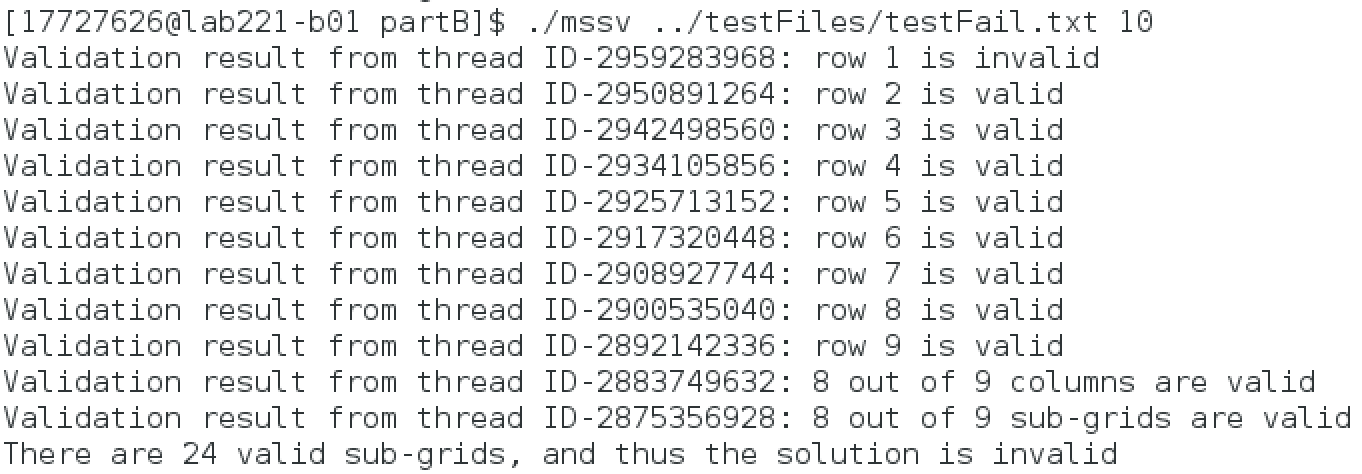
\includegraphics[height=0.25\textheight,width=1.0
			\textwidth]{Thr_testF.png}}
	\end{center}
	\end{figure}

	\begin{figure}[H]
	\caption{Processes: multiFail}
	\begin{center}
		{
			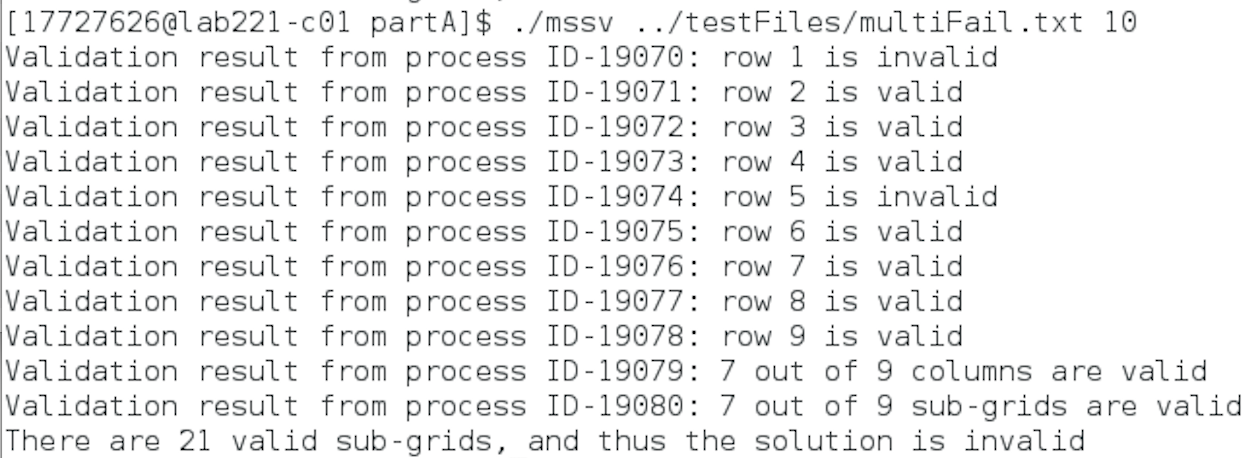
\includegraphics[height=0.25\textheight,width=1.0
			\textwidth]{Pro_multiF.png}}
	\end{center}
	\end{figure}


	\begin{figure}[H]
	\caption{Threads: multiFail}		
	\begin{center}
		{
			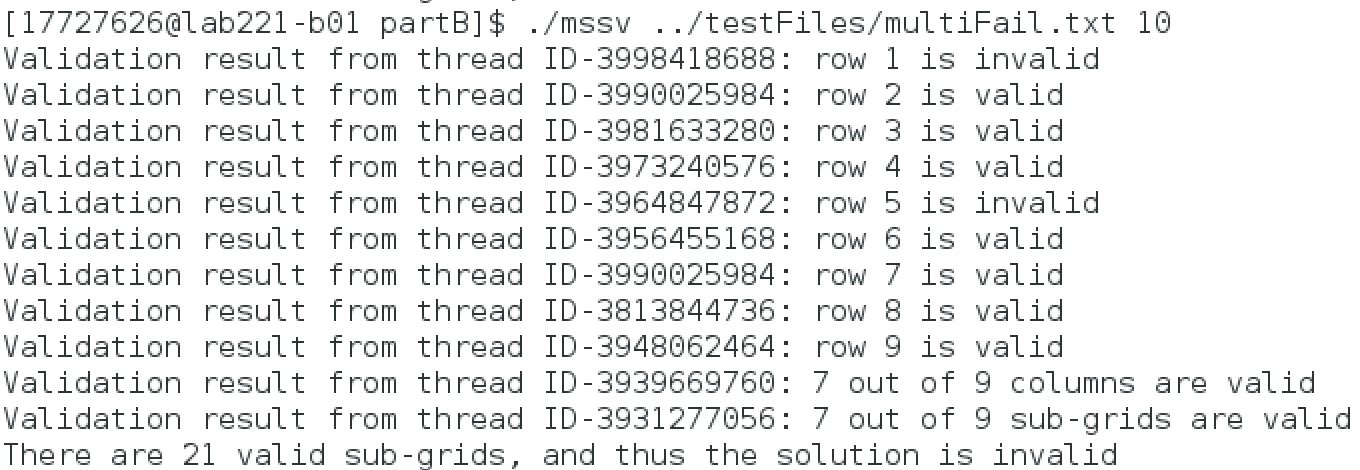
\includegraphics[height=0.25\textheight,width=1.0
			\textwidth]{Thr_multiF.png}}
	\end{center}
	\end{figure}

\pagebreak

%--------------------------------------------------------
% README
\section{README}



\subsection{Purpose}
The program validates an input file containing a sudoku solution. There are two versions. One utilising processes and the other utilising threads.

\subsection{Running the Program}
To compile the C files into an executable format.

\begin{lstlisting}[style=code]
	make
\end{lstlisting}

To run the program there are two options.\\

Option 1:


\begin{lstlisting}[style=code]
	make run 
\end{lstlisting}
\vspace{0.5cm}
This will only let you run with the preset parameters and they will need to be altered in the Makefile to test other \textit{input files} and \textit{delays} 


\begin{lstlisting}[style=code]
INPUT: ../testFiles/specTest.txt
DELAY: 10
\end{lstlisting}
\vspace{0.5cm}
Option 2: 
\begin{lstlisting}[style=code]
./mssv <inputFile> <delay>
\end{lstlisting}

\vspace{0.5cm}
Between each time the program is run, the following command should be entered and executed. This is to delete the logfile produced from an invalid test file.

\begin{lstlisting}[style=code]
	make clean
\end{lstlisting}

\subsection{Files}
partA
\begin{itemize}
	\item Makefile
	\item mssv.c
	\item mssv.h
\end{itemize}

partB
\begin{itemize}
	\item Makefile
	\item mssv.c
	\item mssv.h
\end{itemize}

testFiles
\begin{itemize}
	\item test files
\end{itemize}

\pagebreak


% REFERENCES
\addcontentsline{toc}{section}{References}

%\bibliographystyle{chicago}
\nocite{*}
\printbibliography
%\bibliography{references}
\pagebreak
%--------------------------------------------------------
% APPENDICES
\section{Appendices}
\subsection{Processes: mssv.c}
\lstinputlisting[language=c]{./mssvA.c}
\pagebreak
\subsection{Processes: mssv.h}
\lstinputlisting[language=c]{../partA/mssv.h}
\pagebreak
\subsection{Processes: Makefile}
\lstinputlisting{../partA/Makefile}
\pagebreak
\subsection{Threads: mssv.c}
\lstinputlisting[language=c]{./mssvB.c}
\pagebreak
\subsection{Threads: mssv.h}
\lstinputlisting[language=c]{../partB/mssv.h}
\pagebreak
\subsection{Threads: Makefile}
\lstinputlisting{../partB/Makefile}

\end{document}          
